\ifx\allfiles\undefined
\documentclass[12pt, a4paper, oneside, UTF8]{ctexbook}
\def\path{../config}
\usepackage{amsmath}
\usepackage{amsthm}
\usepackage{array}
\usepackage{amssymb}
\usepackage{graphicx}
\usepackage{mathrsfs}
\usepackage{enumitem}
\usepackage{geometry}
\usepackage[colorlinks, linkcolor=black]{hyperref}
\usepackage{stackengine}
\usepackage{yhmath}
\usepackage{extarrows}
% \usepackage{unicode-math}
\usepackage{esint}
\usepackage{multirow}
\usepackage{fancyhdr}
\usepackage[dvipsnames, svgnames]{xcolor}
\usepackage{listings}
\usepackage{float} % Required for the H float option
\definecolor{mygreen}{rgb}{0,0.6,0}
\definecolor{mygray}{rgb}{0.5,0.5,0.5}
\definecolor{mymauve}{rgb}{0.58,0,0.82}
\definecolor{NavyBlue}{RGB}{0,0,128}
\definecolor{Rhodamine}{RGB}{255,0,255}
\definecolor{PineGreen}{RGB}{0,128,0}

\graphicspath{ {figures/},{../figures/}, {config/}, {../config/} }

\linespread{1.6}

\geometry{
    top=25.4mm, 
    bottom=25.4mm, 
    left=20mm, 
    right=20mm, 
    headheight=2.17cm, 
    headsep=4mm, 
    footskip=12mm
}

\setenumerate[1]{itemsep=5pt,partopsep=0pt,parsep=\parskip,topsep=5pt}
\setitemize[1]{itemsep=5pt,partopsep=0pt,parsep=\parskip,topsep=5pt}
\setdescription{itemsep=5pt,partopsep=0pt,parsep=\parskip,topsep=5pt}

\lstset{
    language=Mathematica,
    basicstyle=\tt,
    breaklines=true,
    keywordstyle=\bfseries\color{NavyBlue}, 
    emphstyle=\bfseries\color{Rhodamine},
    commentstyle=\itshape\color{black!50!white}, 
    stringstyle=\bfseries\color{PineGreen!90!black},
    columns=flexible,
    numbers=left,
    numberstyle=\footnotesize,
    frame=tb,
    breakatwhitespace=false,
} 

\lstset{
    language=TeX, % 设置语言为 TeX
    basicstyle=\ttfamily, % 使用等宽字体
    breaklines=true, % 自动换行
    keywordstyle=\bfseries\color{NavyBlue}, % 关键字样式
    emphstyle=\bfseries\color{Rhodamine}, % 强调样式
    commentstyle=\itshape\color{black!50!white}, % 注释样式
    stringstyle=\bfseries\color{PineGreen!90!black}, % 字符串样式
    columns=flexible, % 列的灵活性
    numbers=left, % 行号在左侧
    numberstyle=\footnotesize, % 行号字体大小
    frame=tb, % 顶部和底部边框
    breakatwhitespace=false % 不在空白处断行
}

% \begin{lstlisting}[language=TeX] ... \end{lstlisting}

% 定理环境设置
\usepackage[strict]{changepage} 
\usepackage{framed}

\definecolor{greenshade}{rgb}{0.90,1,0.92}
\definecolor{redshade}{rgb}{1.00,0.88,0.88}
\definecolor{brownshade}{rgb}{0.99,0.95,0.9}
\definecolor{lilacshade}{rgb}{0.95,0.93,0.98}
\definecolor{orangeshade}{rgb}{1.00,0.88,0.82}
\definecolor{lightblueshade}{rgb}{0.8,0.92,1}
\definecolor{purple}{rgb}{0.81,0.85,1}

\theoremstyle{definition}
\newtheorem{myDefn}{\indent Definition}[section]
\newtheorem{myLemma}{\indent Lemma}[section]
\newtheorem{myThm}[myLemma]{\indent Theorem}
\newtheorem{myCorollary}[myLemma]{\indent Corollary}
\newtheorem{myCriterion}[myLemma]{\indent Criterion}
\newtheorem*{myRemark}{\indent Remark}
\newtheorem{myProposition}{\indent Proposition}[section]

\newenvironment{formal}[2][]{%
	\def\FrameCommand{%
		\hspace{1pt}%
		{\color{#1}\vrule width 2pt}%
		{\color{#2}\vrule width 4pt}%
		\colorbox{#2}%
	}%
	\MakeFramed{\advance\hsize-\width\FrameRestore}%
	\noindent\hspace{-4.55pt}%
	\begin{adjustwidth}{}{7pt}\vspace{2pt}\vspace{2pt}}{%
		\vspace{2pt}\end{adjustwidth}\endMakeFramed%
}

\newenvironment{definition}{\vspace{-\baselineskip * 2 / 3}%
	\begin{formal}[Green]{greenshade}\vspace{-\baselineskip * 4 / 5}\begin{myDefn}}
	{\end{myDefn}\end{formal}\vspace{-\baselineskip * 2 / 3}}

\newenvironment{theorem}{\vspace{-\baselineskip * 2 / 3}%
	\begin{formal}[LightSkyBlue]{lightblueshade}\vspace{-\baselineskip * 4 / 5}\begin{myThm}}%
	{\end{myThm}\end{formal}\vspace{-\baselineskip * 2 / 3}}

\newenvironment{lemma}{\vspace{-\baselineskip * 2 / 3}%
	\begin{formal}[Plum]{lilacshade}\vspace{-\baselineskip * 4 / 5}\begin{myLemma}}%
	{\end{myLemma}\end{formal}\vspace{-\baselineskip * 2 / 3}}

\newenvironment{corollary}{\vspace{-\baselineskip * 2 / 3}%
	\begin{formal}[BurlyWood]{brownshade}\vspace{-\baselineskip * 4 / 5}\begin{myCorollary}}%
	{\end{myCorollary}\end{formal}\vspace{-\baselineskip * 2 / 3}}

\newenvironment{criterion}{\vspace{-\baselineskip * 2 / 3}%
	\begin{formal}[DarkOrange]{orangeshade}\vspace{-\baselineskip * 4 / 5}\begin{myCriterion}}%
	{\end{myCriterion}\end{formal}\vspace{-\baselineskip * 2 / 3}}
	

\newenvironment{remark}{\vspace{-\baselineskip * 2 / 3}%
	\begin{formal}[LightCoral]{redshade}\vspace{-\baselineskip * 4 / 5}\begin{myRemark}}%
	{\end{myRemark}\end{formal}\vspace{-\baselineskip * 2 / 3}}

\newenvironment{proposition}{\vspace{-\baselineskip * 2 / 3}%
	\begin{formal}[RoyalPurple]{purple}\vspace{-\baselineskip * 4 / 5}\begin{myProposition}}%
	{\end{myProposition}\end{formal}\vspace{-\baselineskip * 2 / 3}}


\newtheorem{example}{\indent \color{SeaGreen}{Example}}[section]
\renewcommand{\proofname}{\indent\textbf{\textcolor{TealBlue}{Proof}}}
\newenvironment{solution}{\begin{proof}[\indent\textbf{\textcolor{TealBlue}{Solution}}]}{\end{proof}}

% 自定义命令的文件

\def\d{\mathrm{d}}
\def\R{\mathbb{R}}
%\newcommand{\bs}[1]{\boldsymbol{#1}}
%\newcommand{\ora}[1]{\overrightarrow{#1}}
\newcommand{\myspace}[1]{\par\vspace{#1\baselineskip}}
\newcommand{\xrowht}[2][0]{\addstackgap[.5\dimexpr#2\relax]{\vphantom{#1}}}
\newenvironment{mycases}[1][1]{\linespread{#1} \selectfont \begin{cases}}{\end{cases}}
\newenvironment{myvmatrix}[1][1]{\linespread{#1} \selectfont \begin{vmatrix}}{\end{vmatrix}}
\newcommand{\tabincell}[2]{\begin{tabular}{@{}#1@{}}#2\end{tabular}}
\newcommand{\pll}{\kern 0.56em/\kern -0.8em /\kern 0.56em}
\newcommand{\dive}[1][F]{\mathrm{div}\;\boldsymbol{#1}}
\newcommand{\rotn}[1][A]{\mathrm{rot}\;\boldsymbol{#1}}

% 修改参数改变封面样式,0 默认原始封面、内置其他1、2、3种封面样式
\def\myIndex{0}


\ifnum\myIndex>0
    \input{\path/cover_package_\myIndex}
\fi

\def\myTitle{标题:一份LaTeX笔记模板}
\def\myAuthor{作者名称}
\def\myDateCover{封面日期: \today}
\def\myDateForeword{前言页显示日期: \today}
\def\myForeword{前言标题}
\def\myForewordText{
    
    这是一个基于\LaTeX{}的模板,用于撰写学习笔记。

    模板旨在提供一个简单、易用的框架,以便你能够专注于内容,而不是排版细节,如不是专业者,不建议使用者在模板细节上花费太多时间,而是直接使用模板进行笔记撰写。遇到问题,再进行调整解决。
}
\def\mySubheading{副标题}


\begin{document}

\else
\fi

\chapter{重力荷载}

\section{结构自重}

\begin{definition}
    构件自重:
\[ G_b = \gamma V \]
结构总自重:
\[ G = \sum_{i=1}^{n} \gamma_i V_i \]
\end{definition}

\section{土压力}

\begin{definition}
    成层土中竖向自重应力沿深度的分布:
$$
\sigma_{cz} = \gamma_1 h_1 + \gamma_2 h_2 + \cdots + \gamma_n h_n = \sum_{i=1}^{n} \gamma_i h_i
$$
如果考虑地下水位的话,存在突变。

具体为,假如到深度$h_1$处为地下水位线,由刚才土自重应力计算公式得,$\sigma_1=\gamma_1 h_1$

地下水位到$h_2$结束,那么$h_2$上端为$\gamma_1 h_1 + (\gamma_2 -\gamma_w )h_2$ (可以理解为去掉了水的浮力)

但是$h_2$下端,突变为$\gamma_1 h_1 + \gamma_2 h_2$ (这里不考虑水的重力了)
\end{definition}

\begin{figure}[H]
    \centering
    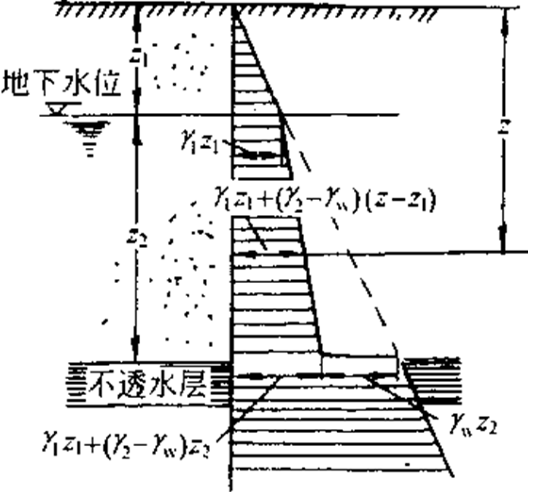
\includegraphics[width=0.5\textwidth]{../figure/tuyali}
    \caption{土压力示意图}
    \label{fig:tuyali}
\end{figure}

\section{雪荷载}

\begin{definition}
    $s = \gamma d = \rho g d$
\begin{enumerate}
    \item $s$: 雪压 ($kN/m^2$)
    \item $d$: 积雪深度,指从积雪表面到地面的垂直深度 (m)
    \item $\gamma$: 雪重度 ($kN/m^3$)
    \item $\rho$: \text{积雪密度 ($kg/m^3$)}
    \item $g$: 重力加速度,取$9.8m/s^2$。
\end{enumerate}
\label{eq:snow_pressure}
\end{definition}

\begin{remark}
    雪荷载喜欢考定义,主要影响因素是雪深和雪重度
\end{remark}

\textbf{雪密度随雪深的变化:}

刚刚飘落的雪十分蓬松,密度较小,大约为:50~100 kg/m³

积雪达到一定厚度时,下层积雪压密,雪密度增加。

\textbf{雪密度随时间的变化:}

积雪反复冻融作用及人为踩踏搅动,其密度也会增加。

\textbf{海拔高度对基本雪压的影响:}

一般基本雪压随海拔高度增加而增大。因为海拔较高的地区温度较低,降雪机会增多且积雪融化延缓。

\begin{remark}
    最大雪深与最大雪密度两者并不一定同时出现。

最好是直接量测雪压,即直接记录地面雪压值。
\end{remark}

\begin{definition}
    基本雪压:

空旷平坦地面上,根据当地气象台观察并收集的年\textbf{最大雪压},经统计得出的50年一遇的最大雪压(即重现期为50年)的概率分布(极值分布),取分布上取某个分位值(\( p_k \)=0.36)为雪压标准值;对雪敏感的结构(主要指大跨、轻质屋盖结构),应采用100年重现期的雪压分布
\end{definition}

基本雪压是针对地面上的积雪荷载定义的。屋面雪荷载由于多种因素影响,往往与地面雪荷载不同。

影响屋面积雪的因素:

风对屋面积雪的影响:漂积作用

屋面形式(坡度)对积雪的影响:雪的滑移,{\color{red}显然坡度越大,屋面雪压力越小}

屋面散热(温度)对积雪的影响:积雪融化、积雪滑移

\begin{definition}
    屋面水平投影面的雪荷载标准值按下式计算:
\[ S_k = \mu_r S_0 \]
\[ S_k \quad \text{—— 雪荷载标准值(kN/m²)} \]
\[ \mu_r \quad \text{—— 屋面积雪分布系数} \]
\[ S_0 \quad \text{—— 地面基本雪压(kN/m²)} \]
\end{definition}

\section{汽车荷载}

\begin{definition}
    汽车荷载分为车道荷载(包含均布荷载和集中荷载)和车辆荷载
\end{definition}

\begin{remark}
    车辆荷载和车道荷载的作用不得叠加
\end{remark}

\begin{figure}[H]
    \centering
    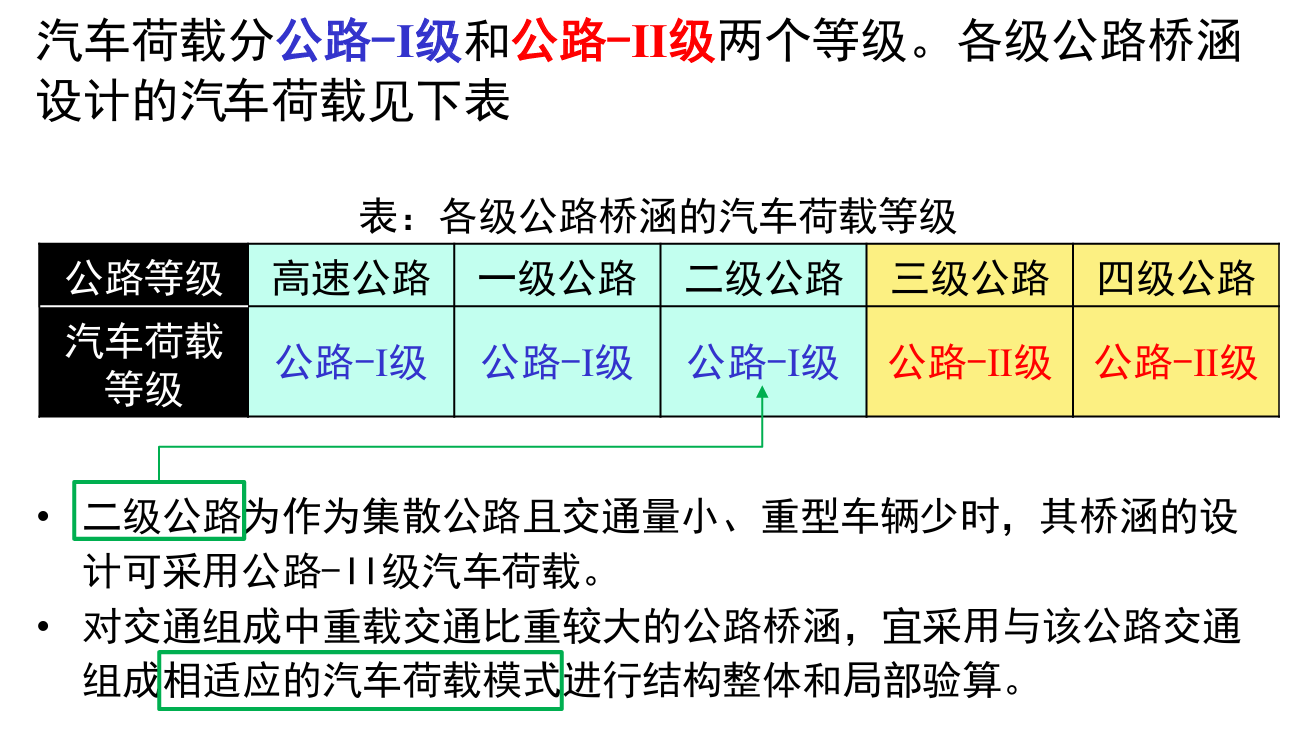
\includegraphics[width=0.8\textwidth]{../figure/qichehezai.png}
    \caption{汽车荷载等级}
    \label{fig:qichehezai}
\end{figure}

\begin{enumerate}
    \item 车辆荷载:考虑车的尺寸及车的排列方式,以集中荷载的形式作用于车轴(即车轮)位置。
    \item 车道荷载:不考虑车的尺寸及排列方式,将其等效为均布荷载和一个可作用于任意位置的集中荷载形式。
    \item 公路Ⅰ级和公路Ⅱ级汽车荷载采用相同的车辆荷载标准值。
    \item 车道荷载是个虚拟荷载,由均布荷载和集中荷载组成。
    \item 对于连续梁,常用影响线辅助寻找产生最不利效应的最不利荷载分布。
    \item 多车道桥梁上的汽车荷载应考虑多车道折减(横向折减)
    \item 大跨径桥梁随着桥梁跨度的增加桥梁上实际通行的车辆达到较高
    密度和满载的概率减小,应考虑纵向计算跨径折减。当为多跨连续结构时,整个结构应按最大的计算
    跨径考虑汽车荷载效应的折减。
\end{enumerate}

\section{楼面活荷载}

\begin{definition}
    活荷载的定义:

指建筑物中的人群、家具、设施等产生的重力作用,这些荷载的量值随时间发生变化,位置也是可移动的,亦称{\color{red}可变荷载}。

楼面活荷载按其随时间变异的特点,可分为持久性和临时性两部分:

\begin{enumerate}
    \item 持久性活荷载:(Sustained live load)是指楼面上在某个时段内基本保持不变的荷载,例如住宅内的家具、常住人员等;
    \item 临时性活荷载:(Transient live load)是指楼面上偶尔出现的短期荷载,例如聚会的人群、装修材料的堆积等。
\end{enumerate}

楼面活荷载一般处理为均布荷载,不同场景的均布荷载计算不同
\end{definition}

\begin{example}
下面结构受到的作用,属于结构自重的是:(B)  

A. 家具的重力;  

B. 楼面板受到的重力;  

C. 人员的重力;  

D. 屋顶积雪的重力。
\end{example}

\begin{remark}
    由我们刚才的讨论可以知道,家具和人员都属于楼面活荷载,设备也是。
\end{remark}

\begin{example}
    计算楼面活荷载时,为什么当活荷载作用面积超过一定数值时,需对楼面活荷载进行折减?

    由于楼面均布活荷载可理解为总活荷载按楼面面积平均,面积越大,平摊的楼面活荷载越小。
\end{example}

\section{人群荷载}

\begin{definition}
    人群荷载分为公路桥梁人群荷载、城市桥梁人群荷载、铁路桥梁人行道荷载

    (暂时不知道啥是重点)
\end{definition}

\ifx\allfiles\undefined
\end{document}
\fi